\chapter{Stworzony model zjawiska}

Niniejszy rozdział opisuje szczegółowo kolejne kroki oraz wykorzystane algorytmy niezbędne do uzyskania efektu końcowego.

%---------------------------------------------------------------------------

\section{Opracowanie danych topograficznych}

\subsection{Wybór cech}
Jak wspomniano już wcześniej, do oszacowania ryzyka lawinowego konieczne jest posiadanie danych dotyczących cech terenu. Bazując na pracy pani Izabeli Woszczak, skupiono się na obliczeniu taki cech, jak:
\begin{itemize}
	\item nachylenie powierzchni;
	\item ekspozycja słoneczna;
	\item piętro;
	\item wysokość;
	\item forma terenu (skupiono się na żlebach).
\end{itemize}

\subsection{Format .las}
Na początkowym etapie pracy otrzymano pliki w formacie .las - każdy z nich reprezentujący ukształtowanie terenu wybranego obszaru. 

Format .las został stworzony do przechowywania zbioru punktów w przestrzeni trójwymiarowej (ang. point cloud), otrzymanych przy pomocy metody Lidar, która polega na oświetlaniu wybranych punktów na powierzchni Ziemi laserem i zapisie jego odbicia przy pomocy sensorów. Dzięki tej metodzie powstają mapy o wysokiej rozdzielczości, stosowane w naukach o Ziemi (Sustainability of Digital Formats: Planning for Library of Congress Collections loc.gov/preservation/digital/formats/fdd/fdd000418, dostęp 7 czerwca 2020). 

Otrzymane pliki zawierały średnio około 11 milionów punktów, przy czym każdy z nich reprezentował powierzchnię około 4 km$^2$.

\begin{figure}[h]
	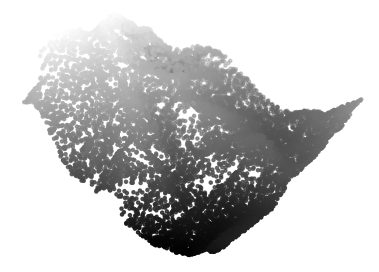
\includegraphics[width=8cm]{las_example}
	\centering
	\caption{Uproszczona wizualizacja zbioru punktów z pliku .las}
\end{figure}

\subsection{Triangulacja Delaunaya}
Sam zbiór punktów nie oferuje możliwości łatwego obliczania wyżej wymienionych cech, dlatego zastosowano uproszczenie powierzchni terenu przy pomocy triangulacji Delaunaya.

Jest to algorytm, który na podstawie zbioru punktów tworzy zbiór trójkątów, gdzie wierzchołki każdego trójkąta stanowią owe punkty. Własnością algorytmu jest, że maksymalizuje on najmniejsze z katów w powstałych trójkątach, unikając tzw. sliver triangles (Delaunay 1934).


\begin{figure}[h]
	\centering
	\begin{minipage}{.5\textwidth}
		\centering
		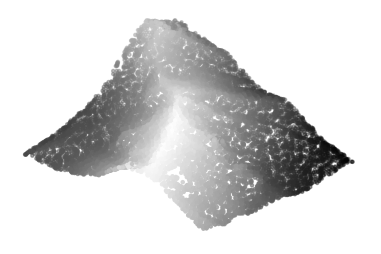
\includegraphics[width=.6\linewidth]{no_delaunay}
		\captionof{figure}{Obszar przedstawiony jako zbiór punktów}
		\label{fig:test1}
	\end{minipage}%
	\begin{minipage}{.5\textwidth}
		\centering
		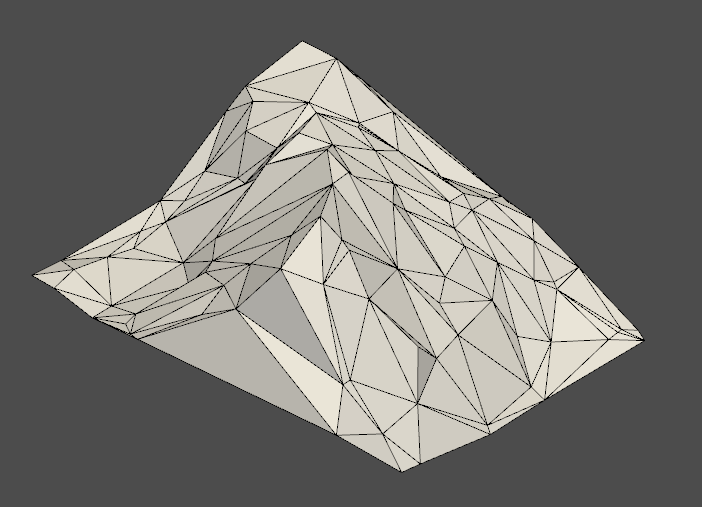
\includegraphics[width=.6\linewidth]{delaunay}
		\captionof{figure}{Ten samo obszar poddany triangulacji}
		\label{fig:test2}
	\end{minipage}
\end{figure}

\subsection{Nachylenie powierzchni i ekspozycja słoneczna}
Uzyskanie trójkątów umiejscowionych w przestrzeni trójwymiarowej (każdy trójkąt reprezentuje krotka 3 punktów $(x, y, z)$) pozwoliło na obliczenie ekspozycji słonecznej oraz nachylenia powierzchni dla każdego z nich przy pomocy odpowiednich operacji algebry liniowej. Kod dla obliczeń przedstawionych w tym podrozdziale został wylistowany w podrodziale ...

\clearpage 

\subsubsection{Obliczenia dla nachylenia powierzchni}
Algorytm obliczania nachylenia powierzchni dla każdego trójkąta (odpowiednie wektory przedstawione są na \textbf{Rys. 2.4.}):

\begin{enumerate}
\item Ustal normę $\boldsymbol{r}$ (wektor jednostkowy prostopadły) do płaszczyzny $xy$. 
\item Oblicz normę do płaszczyzny trójkąta wybierając 2 dowolne wektory $\boldsymbol{u}$ i $\boldsymbol{v}$ łączące wierzchołki trójkąta, obliczając iloczyn wektorowy i normalizując go do wektora $\boldsymbol{n}$.
\item Oblicz iloczyn skalarny dla normy płaszczyzny $xy$ i normy płaszczyzny trojkąta.
\item Oblicz $arccos$ obliczonego iloczynu skalarnego.
\end{enumerate} 

Wynikiem algorytmu jest nachylenie płaszczyzny trójkąta do płaszczyzny $xy$ wyrażone w stopniach.

\begin{figure}[h]
	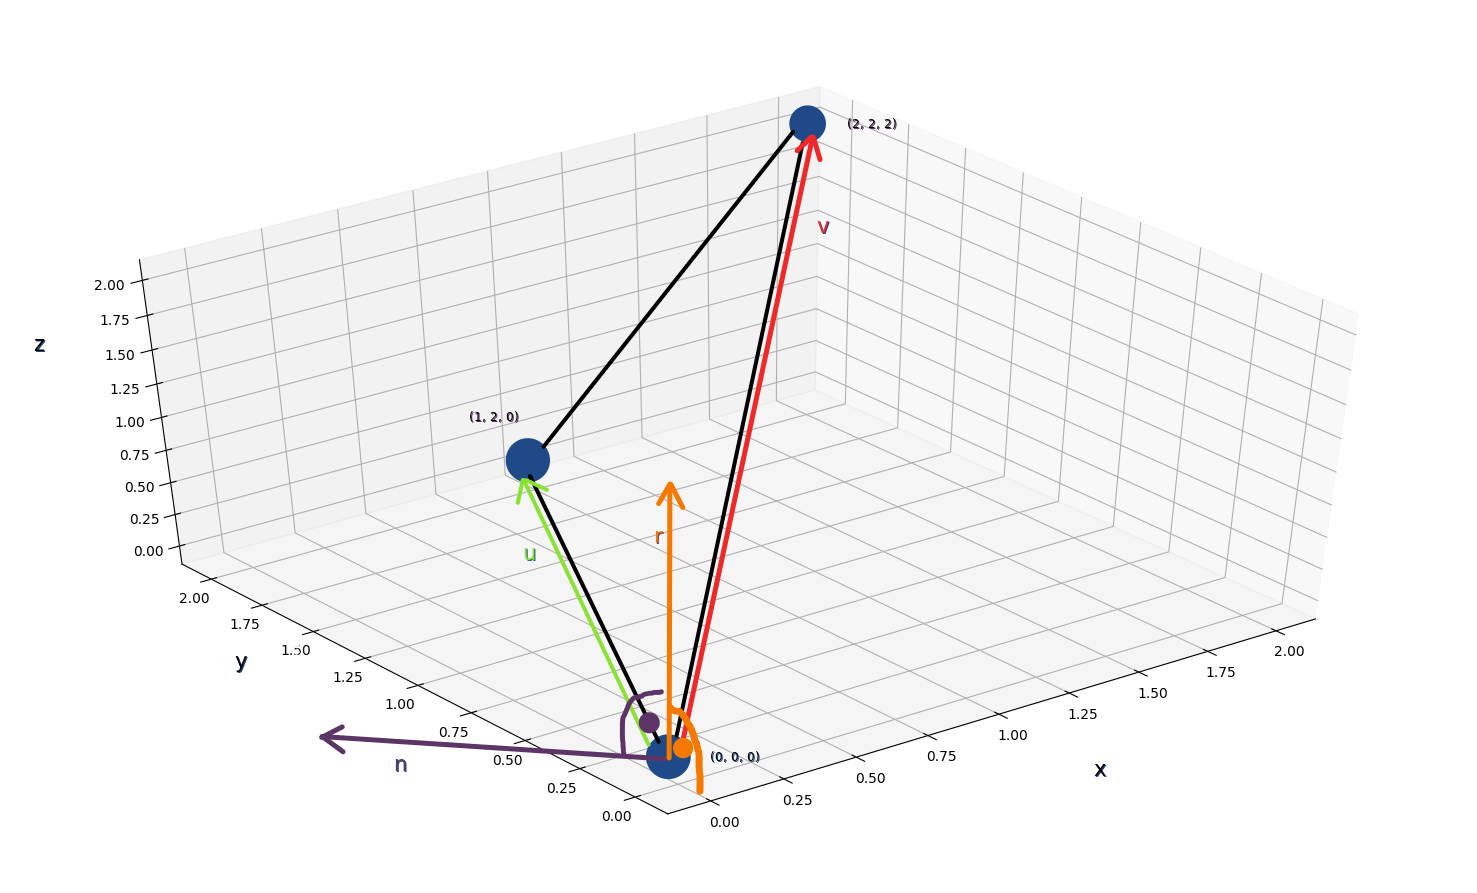
\includegraphics[width=8cm]{vectors}
	\centering
	\caption{Przedstawienie odpowiednich wektorów dla pojedynczego trójkąta}
\end{figure}

\subsubsection{Obliczenia dla ekspozycji słonecznej}
Algorytm obliczania ekspozycji słonecznej przebiega podobnie do algorytmu obliczania nachylenia powierzchni. Każdemu kierunkowi geograficznemu (północ, północny-wschód itd.) odpowiada wektor jednostkowy. Algorytm jest przeprowadzany dla każdego trójkąta i dla każdego kierunku. Jeżeli otrzymany wynik jest mniejszy lub równy 15\degree dla wybranego kierunku, to przyjmuje się, że dany trójkąt reprezentuje stok o wybranej ekspozycji.

\begin{enumerate}
	\item Oblicz normę do płaszczyzny trójkąta wybierając 2 dowolne wektory łączące wierzchołki trójkąta, obliczając iloczyn wektorowy i normalizując go.
	\item Zrzutuj obliczoną normę na płaszczyznę $xy$.
	\item Oblicz iloczyn skalarny dla normy płaszczyzny $xy$ i zrzutowanej normy płaszczyzny trojkąta.
	\item Oblicz $arccos$ obliczonego iloczynu skalarnego.
	\item Jeżeli obliczony kąt jest mniejszy lub równy 15\degree, to przyjmij obecny kierunek jako ekspozycję stoku.
\end{enumerate} 

\subsection{Piętro}
Jak podaje ..., piętra zwiększające ryzyko zejścia lawiny to piętra subalpejskie i alpejskie. Zależą one bezpośrednio od wysokości, którą odczytano bezpośredni z plików .las.

\subsection{Wysokość}
... również określa wysokości, na których najczęściej dochodzi do zejścia lawin. Punkty odczytano bezpośrednio z plików .las.

\subsection{Wklęsłe formy terenu}
Informacje o występowaniu na obszarach jednostkowych żlebów, będących reprezentami wklęsłych form terenu, uzyskano nie na podstawie zawartości plików .las, lecz na podstawie zawartości rządowych witryn internetowych, skąd pliki te zostały pozyskane.

Dzięki zastosowaniu takiego podejścia, zachowano czas na dopracowanie innych elementów symulacji przy zachowaniu 100 PROCENT dokładności w kwestii identyfikacji tak ważnych przy określaniu ryzyka lawinowego form terenu, jak żleby.
 
Korzystając z narzędzi do automatyzacji przeszukiwania kodu HTML, zidentyfikowano ewentualne występowanie żlebów. 


%---------------------------------------------------------------------------

\section{Dane pogodowe}

\subsection{Najważniejsze czynniki}
Dane pogodowe są kolejnymi kluczowymi danymi potrzebnymi do predykcji wystąpienia lawiny na danym obszarze (Joshi, Kumar, Srivastava, Sachdeva, Ganju 2018). Z dostępnych pomiarów wyodrębnione zostały 4 najważniejsze cechy wpływające na występowanie lawiny:
\begin{itemize}
	\item grubość pokrywy śnieżnej;
	\item zmiany temperatury;
	\item opad deszczu;
	\item prędkość wiatru.
\end{itemize}

\subsection{Pobieranie danych pogodowych}
Do pobrania danych pogodowych skorzystano z ogólnodostępnego API z Open Weather Map, umożliwiającego szybkie i częste pobieranie danych pogodowych o wysokiej dokładności.

%--------------------------------------------------------------------------

\section{Predykcja zagrożenia na podstawie danych}
Jak wspomniano w podrodziale 1.3, z powodu braku dostępnych danych charakteryzujących szczegółowo oraz na przestrzeni długiego czasu zjawisko schodzenia lawin, zdecydowano się oprzeć na wnioskach autorów publikacji i w modelu uwzględnić czynniki:
\begin{itemize}
	\item opisane przez autorów jako krytyczne dla zagrożenia;
	\item możliwe do obliczenia lub ustalenia.
\end{itemize}

\subsection{Przyjmowane wartości}
Ostatecznie każdy obszar jednostkowy scharakteryzowano rekordem o następujących cechach (każda przyjmuje jedynie wartości $True$ i $False$, gdzie wartość $True$ oznacza, że cecha przyjmowała wartości zwiększające zagrożenie; wartość $False$ natomiast oznacza, że cecha przyjmowała wartości zmniejszające zagrożenia):
\begin{center}
	\begin{tabular}{|c|c|} 
		\hline
		Nazwa cechy & $True$, gdy \\ 
		\hline
		form\_terenu & na obszarze znajduje się co najmniej 1 żleb. \\ 
		eksp\_sloneczna & na obszarze znajdują się stoki o nachyleniu w przedziale [30\degree, 40\degree] i ekspozycji NE, W lub E. \\
		nachylenie & $ Q_1 \geq 25$\degree \:i\: $ Q_3 \leq 50$\degree. \\
		pietro & max\_wysokość $\geq$ 1600 m n.p.m. \\
		wysokosc & $ Q_1 \geq$ 1300 m n.p.m \:i\: $ Q_3 \leq$ 2100 m n.p.m. \\
		pora\_roku & obecną porą roku jest lato. \\ 
		deszcz48h & w ciągu ostatnich 48 godzin wystąpił opad o minimalnej intensywności 10mm/h. \\
		snieg48h & w ciągu ostatnich 48 godzin opad śniegu przekroczył próg 200mm. \\
		wiatr48h & w ciągu ostatnich 48 godzin wystąpił wiatr o minimalnej prędkości 13m/s. \\
		wzr\_temp & w ciągu ostatnich 48 godzin temperatura zmieniła się z ujemnej na dodatnią i $t\_śr$ > 0\degree. \\
		\hline
	\end{tabular}
\end{center}

\subsection{Uzasadnienie przyjętych wartości}
Wartości graniczne, które decydują, czy dana cech przyjmie wartość zwiększającą ($True$), czy zmniejszającą zagrożenie ($False$), zostały przyjęte zgodnie z treścią przeanalizowanych publikacji naukowych:
\begin{itemize}
	\item forma terenu - \textit{"Istotnym czynnikiem sprzyjającym wystąpieniu lawiny jest forma terenu. Kształt stoku ma bowiem wpływ na grubość odkładanej warstwy śniegu, co bezpośrednio wiąże się ze wzrostem zagrożenia lawinowego. (...) Największe zagrożenie lawinowe obejmuje stoki wklęsłe w profilu poprzecznym doliny, przede wszystkim żleby i jary."}\;(Woszczek 2016)
	\item ekspozycja słoneczna - \textit{"Analiza i charakterystyka ekspozycji terenu przeprowadzona dla wybranych uśrednionych wartości ekspozycji wykazała, że w badanej próbie największy udział mają ekspozycje północno-wschodnia, wschodnia oraz zachodnia, łącznie stanowiące 75\% analizowanych przypadków."}\;(Woszczek 2016)
	\item nachylenie - \textit{"Za najistotniejszy wskaźnik uznano średnią wartość nachylenia. Spośród dwudziestu analizowanych przypadków dla piętnastu z nich (75\%) średnie wartości nachyleń odpowiadają przedziałowi od 30\degree do 40\degree (...) krytycznym kącie nachylenia terenu, który został określony na podstawie wieloletnich obserwacji lawin. Przedział wartości tego kąta wynosi od 20 do 50\degree \;(IMGW–PIB)."}\;(Woszczek 2016) oraz \textit{"Most avalanches occur on the hillside with a slope angle of about 36\degree to 42\degree."}\;(Hao, Huang, Liu, Amanambu, Li 2018)
	\item piętro - \textit{"I tak, w przypadku wysokości minimalnych do piętra subalpejskiego i alpejskiego zaliczono łącznie 80\% przypadków, a pozostałe 20\% wystąpiło w piętrze leśnym."}\;(Woszczek 2016)
	\item wysokość - \textit{"Większe znaczenie mają obliczone wartości najmniejszych i największych wysokości maksymalnych oraz minimalnych. (...) Największa maksymalna wysokość została przypisana lawinie w rejonie Buli pod Rysami – 2094 m n.p.m., a najmniejsza – tej w rejonie Małego Kotła
	Mięguszowieckiego – 1625 m n.p.m. Najmniejsza wysokość minimalna obliczona została dla wspomnianej już największej lawiny (która miała miejsce w Krówskim Żlebie) – i wyniosła 1363 m n.p.m. Największa natomiast była dla lawiny spod Pośredniego Wierchu Goryczkowego – 1888 m n.p.m."} (Woszczek 2016)
	\item pora roku - okres zimowy przyjęto jako niebezpieczny z powodu ujemnych temperatur i dużych opadów śniegu. \textit{"W okresie jesiennym lawiny gruntowe tworzy pierwsza, cienka warstwa śniegu, która zsuwa się wzdłuż powierzchni stoku, odsłaniając podłoże pozbawione pokrywy śnieżnej."} oraz \textit{"W okresie wiosennym pojawianie się lawin gruntowych związane jest ze wzrostem temperatury i opadami deszczu, które powodują topnienie, a co za tym idzie – wzrost ciężaru śniegu."} (Woszczek 2016)
	\item wzrost temperatury - \textit{"There is a high probability of temperature-rise-triggered avalanche release when temperature continuously rises within three days and daily mean temperature in the following day reaches 0.5\degree C in late February to mid-March."} (Hao i in. 2018)
\end{itemize}
	Wartości dotyczące opadów śniegu oraz wiatru przyjęto na podstawie wskazań Górskiego Pogotowia Ratunkowego w Słowacji (laviny.sk/metodika-laviny/nauka-o-snehu-a-lavinach, dostęp 7 czerwca 2020).
	
	Nie znaleziono wartości dotyczących opadów śniegu - jedynym punktem odniesienia jest informacja, iż opad musi być intensywny, aby przyczynić sie do powstania lawiny. 

\subsection{Syntetyczny zbiór danych}
Jak wspomniano w sekcji 1.3, obecnie na świecie rozwiązania są oparte niemal wyłącznie na metodach statystycznych oraz metodach uczenia maszynowego, które wymagają odpowiednich danych.

Postanowiono wieć stworzyć własny zbiór danych w sposób sztuczny, aby następnie na ich podstawie utworzyć odpowiednie drzewo decyzyjne. Takie podejście pozwala wprowadzić reguły zaczerpnięte z publikacji, jednocześnie budująć fundament prawdziwego rozwiązania. 

Kolejne kroki tworzenia sztucznego zbioru to:
\begin{enumerate}
	\item Uzyskanie wszystkich możliwych kombinacji cech (z pominięciem powstałych rekordów, które są wewnętrznie sprzeczne).
	\item Przypisanie rekordom odpowiednich etykiet odpowiadających stopniowi zagrożenia. 
\end{enumerate}

Etykiety dobrano uważnie analizując wybrane publikacje i zwracając uwagę na nacisk autorów przy wymienianiu kolejnych czynników tworzących zagrożenie. Najwyższą rolę przypisano porze roku oraz opadom śniegu w ciągu 48 godzin. Zagrożenie wysokie przypisano rekordom przyjmującym dla cech niemal same wartości $True$.

\begin{center}
	\begin{tabular}{|c|c|} 
		\hline
		Spełnione warunki & Zagrożenie \\ 
		\hline
		form\_terenu = $False$ AND wysokosc = $False$ & brak \\
		\hline
		pora\_roku = $False$ AND snieg48h = $False$  & brak \\
		\hline
		deszcz48h = $False$ AND snieg48h = $False$ AND wiatr48h = $False$ AND wzr\_temp = $False$ & brak \\
		\hline 
		form\_terenu = $True$ AND ....
		
	\end{tabular}
\end{center}

W efekcie powstały 1024 rekordy, na podstawie których zbudowano drzewo decyzyjne.
\subsection{Drzewo decyzyjne}
Napisać o zaletach (źródło), przedstawić wynikowe drzewo.
